\subsubsection{Reverberation}
\label{sec:reverb-discussion}

In acoustics, Artificial Reverberation simulates the reflection of sounds in all directions
in a closed, airtight room, eventually giving the audio a prolonged sound in the simulated
environment. These reflections occur spontaneously, thus giving endless amount of echoes superposing
each other. Algorithmic reverb will be implemented in this project, which consists of methodologies
like Freeverb, Dattoro, Lexverb, Feedback Delay Network (FDN), etc. \cite{valimaki2012fifty, fluidsynth_reverb_overview}

But due to such spontaneity, there is no right or wrong solution as to what kind of algorithmic reverb 
can be used. Therefore, Signalsmith's Reverb is chosen as the solution to designing the reverb,
which is simply the modified version of the FDN reverberation algorithm \cite{smith2010pasp}. FluidSynth recently introduced this 
algorithm in their latest version 2.6.0, and produces the most realistic sound, although computationally 
expensive \cite{fluidsynth_reverb_overview}.

Geriant Luff's blog page, ``How to Write a Reverb'' is used to design the algorithm for creating Signalsmith's Reverb.
The following figure below shows the block diagram of the architecture for Signalsmith's Reverberation
at the initial stage taken from the blog \cite{luff2021reverb}.

\begin{figure}[ht]
  \centering
  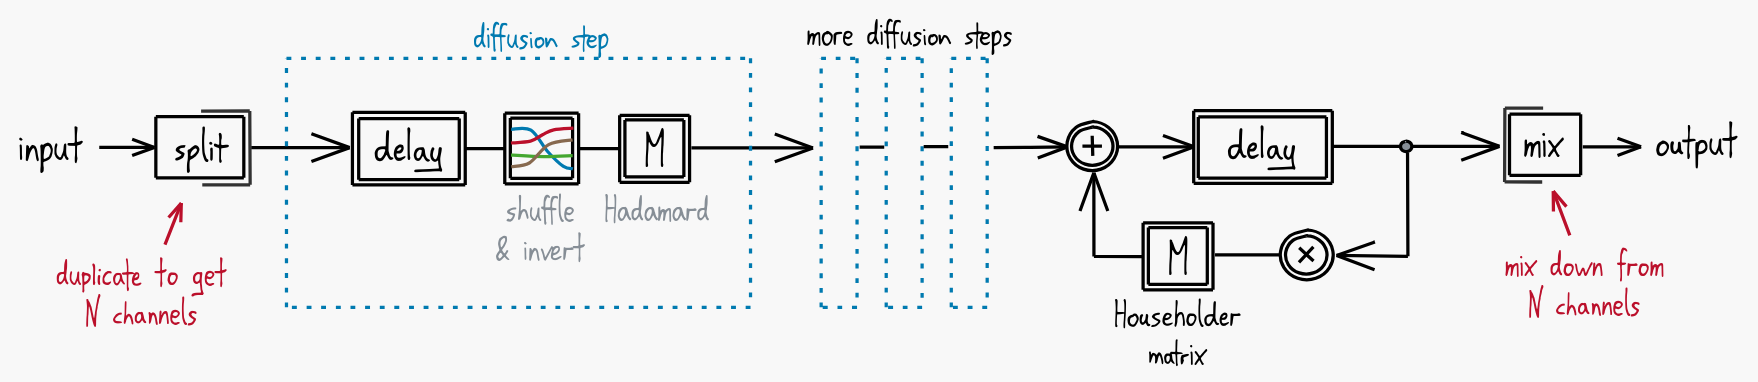
\includegraphics[width=\linewidth]{discussion/audio_effects/reverb/figures/signalsmith_diagram.png}
  \caption{Architecture of the minimalistic design of the architecture \cite{luff2021reverb}} % TODO: Change the citation
  \label{fig:signalsmith}
\end{figure}


The Signalsmith's algorithm consists of the following stages \cite{luff2021reverb}:
\begin{enumerate}
    \item \textbf{Split}: This simply duplicates the signal to 4, 8, or 16 channels.
    \item \textbf{Diffusion Stage}: This system consists of multi-channel delay, permutation-polarity change, 
    and the Hadamard transform \cite{smith2010pasp}. After the multi-channel signal passes through multiple 
    diffusion stages, the echo becomes more densely packed, thus making the dry audio sound blurred.
    \item \textbf{Multi-channel Comb Filter}: This simply creates echo, with a decay gain, where $0 \leq g < 1$. It has
    the same multi-channel delay as in the Diffusion stage, but with different delay times. It also uses a 
    Householder matrix \cite{higham2020householder} as a mixing matrix in the feedback path to prevent 
    such identifiable patterns from being recognized.
\end{enumerate}

To understand the subsystems, the following list utilizes some all-pass filters \cite{luff2021reverb}:
\begin{itemize}
    \item \textbf{Multi-channel Delay}: Applies a forward time-shift to the output. The delay times are distinct and randomized
    for each channel, thus producing a spontaneous echo effect from all directions. 
    \item \textbf{Shuffling channels and inverting polarity}: Simply shuffles the channels, and then some of the 
    amplitudes are inverted through natural selection of the channels.
    \item \textbf{Mixing matrix}: Applies linear transformation to the multi-channel signal input and produces
    a different kind of output. These orthogonal matrices must conserve energy such that the amplitudes of the
    resulting output is the same as the input. The system utilizes the Hadamard Matrix \cite{smith2010pasp} 
    and the Householder Matrix \cite{higham2020householder} used in the diffusers and the feedback loop respectively.
\end{itemize}

A multi-channel delay is described by the following equation \cite{smith2010pasp}:

\begin{equation}\label{eq:delay}
y_i[n] = x_i[n - M_i]
\end{equation}

% TODO: Forgotten to put the equation for the choice of delay times d = 4V/s from Schroeder's paper

Where $i$ is the channel number ($i \in \mathbb{Z}^{+}$), $n$ is the sample number ($n \in \mathbb{Z}^{+}$), and
$M$ is the delay time (in samples). They should be mutually prime with each other, which prevents periodic coincidence with 
the signals and metallic ringing, thus maximizing echo spread for each signal, increasing echo density. The delay time will 
be given in milliseconds, so this needs to be converted to samples using the following equation in DSP.

\begin{equation}\label{eq:ms_to_samples}
n = \frac{T_{milli}}{f_s} \times 1000
\end{equation}

Where $T_{milli}$ is the time in milliseconds, and $f_s$ is the sample frequency.

The equations (\ref{eq:hadamard}) and (\ref{eq:householder-general}) below shows the recursive approach to Hadamard matrix \cite{smith2010pasp}
and the Householder Matrix \cite{higham2020householder} respectively.

\begin{equation}\label{eq:hadamard}
    \mathbf{H}_1 = \begin{bmatrix} 1 \end{bmatrix}, \qquad
    \mathbf{H}_{2N} = \begin{bmatrix} H_N & H_N \\ H_N & -H_N \end{bmatrix}
\end{equation}

This needs to be normalized to preserve energy. Therefore,
\begin{equation}\label{eq:hadamard_norm}
    \hat{H}_N = \frac{1}{\sqrt{N}}H_N
\end{equation}

For example, for 4 channels,
$$
    H_4 = \begin{bmatrix}
        1 & 1 & 1 & 1 \\
        1 & -1 & 1 & -1 \\
        1 & 1 & -1 & -1 \\
        1 & -1 & -1 & 1
    \end{bmatrix}, \qquad
    \hat{H}_4 = \frac{1}{2}\begin{bmatrix}
        1 & 1 & 1 & 1 \\
        1 & -1 & 1 & -1 \\
        1 & 1 & -1 & -1 \\
        1 & -1 & -1 & 1
    \end{bmatrix}
$$

The Householder matrix of size $n$, is described by the following \cite{higham2020householder}:
\begin{equation}\label{eq:householder-general}
    \mathbf{P}_n = I - \frac{2}{n} \mathbf{v} \mathbf{v}^T
\end{equation}

% TODO: Please change this inline equation to syntactically correct code
Where $\mathbf{v} = [1, 1, \dots, 1]^T \in \mathbb{R}^n$, a vector of size $n$ containing all 1's. The example below shows this matrix with
4 channels:

$$
    \mathbf{P}_4 = \begin{bmatrix}
        0.5 & -0.5 & -0.5 & -0.5 \\
        -0.5 & 0.5 & -0.5 & -0.5 \\
        -0.5 & -0.5 & 0.5 & -0.5 \\
        -0.5 & -0.5 & -0.5 & 0.5
    \end{bmatrix}
    \label{eq:householder}
$$

The output is obtained by multiplying the matrix with a multi-channel signal $x \in \mathbb{R}^n$, i.e., $y = Mx$, where
$M$ is one of those matrices.

\Cref{fig:fdn_combfilter} shows the $N$-order Feedback-Delay section derived from the FDN system equipped with a series
of IIR Comb Filters. It performs after the system the diffusers finish processing the signals. The feedback utilizes the Householder
matrix in the feedback loop, and reduces the amplitude by applying some gains for each of the system.

\usetikzlibrary{calc}
\begin{figure}[ht]
    \centering
\begin{tikzpicture}

% Delay 1
\node[draw,
    fill=yellow!20,
    minimum width=4cm,
    minimum height=0.8cm,
] (delay1) at (0,0){$z^{-M_1}$};

\draw[-{Stealth[length=3mm]}] ([xshift=-5cm,yshift=0]delay1.west) -- (delay1.west);
\draw[-{Stealth[length=3mm]}] (delay1.east) -- ([xshift=4cm,yshift=0]delay1.east);

% Delay 2
\node[draw,
    fill=yellow!20,
    minimum width=4cm,
    minimum height=0.8cm,
    below=0.6cm of delay1
] (delay2) {$z^{-M_2}$};

\draw[-{Stealth[length=3mm]}] ([xshift=-5cm,yshift=0]delay2.west) -- (delay2.west);
\draw[-{Stealth[length=3mm]}] (delay2.east) -- ([xshift=4cm,yshift=0]delay2.east);

% Vertical Dots
\node[below=0cm of delay2] (box_dots1) {$\vdots$};
\node[below left=0cm and 1.9cm of delay2] (box_dots2) {$\vdots$};
\node[below right=0cm and 1.9cm of delay2] (box_dots3) {$\vdots$};


% Delay N
\node[draw,
    fill=yellow!20,
    minimum width=4cm,
    minimum height=0.8cm,
    below=0.1cm of box_dots1
] (delayN) {$z^{-M_N}$};

\draw[-{Stealth[length=3mm]}] ([xshift=-5cm,yshift=0]delayN.west) -- (delayN.west);
\draw[-{Stealth[length=3mm]}] (delayN.east) -- ([xshift=4cm,yshift=0]delayN.east);

% Input and output labels with braces
\draw[decorate, decoration={brace, amplitude=8pt}, thick]
    ([xshift=-5.2cm]delay1.west |- delayN.west) -- ([xshift=-5.2cm]delayN.west |- delay1.west)
    node[midway, left=8pt] {$x[n]$};

\draw[decorate, decoration={brace, amplitude=8pt, mirror}, thick]
    ([xshift=4.2cm]delay1.east |- delayN.east) -- ([xshift=4.2cm]delayN.east |- delay1.east)
    node[midway, right=8pt] {$y[n]$};


% Matrices
\node[draw,
    fill=blue!20,
    minimum width=2.5cm,
    minimum height=2cm,
    below=1cm of delayN.south,
    inner sep=0cm
] (hadamard) {\shortstack{Householder \\ $\mathbf{P}_n$}};

\draw[-{Stealth[length=3mm]}] ([xshift=-5cm,yshift=0]delay1.west) -- (delay1.west);
\draw[-{Stealth[length=3mm]}] (delay1.east) -- ([xshift=4cm,yshift=0]delay1.east);


% Dots
\node[draw, circle, minimum size=0.2cm, fill=black, inner sep=0cm, right=3.0cm of delay1] (hp_dot1) {};
\node[draw, circle, minimum size=0.2cm, fill=black, inner sep=0cm, right=2.5cm of delay2] (hp_dot2) {};
\node[draw, circle, minimum size=0.2cm, fill=black, inner sep=0cm, right=1.5cm of delayN] (hp_dotN) {};

% Adders
\node[draw, circle, minimum size=0.5cm, inner sep=0cm, fill=red!50, right=-4.3cm of delay1.west] (sum1) {$+$};
\node[draw, circle, minimum size=0.5cm, inner sep=0cm, fill=red!50, right=-3.6cm of delay2.west] (sum2) {$+$};
\node[draw, circle, minimum size=0.5cm, inner sep=0cm, fill=red!50, right=-2.8cm of delayN.west] (sumN) {$+$};





% % small downward triangle labeled 2R below integrator2
% \node[draw,
%     isosceles triangle,
%     shape border rotate=270,
%     minimum size=0.8cm,
%     fill=yellow!20,
%     below=1.2cm of bp_dot,
%     label={[yshift=-2mm]right:2R}
% ] (scalar_R) {};





% Connections
\draw[-{Stealth[length=3mm, width=2mm]}]
    (hp_dot2.south) |- (hadamard.east);

\draw[-{Stealth[length=3mm, width=2mm]}]
    (hp_dot1.south) |- ($(hadamard.east)+(0,0.5cm)$);

\draw[-{Stealth[length=3mm, width=2mm]}]
    (hp_dotN.south) |- ($(hadamard.east)-(0,0.5cm)$);

\draw[-{Stealth[length=3mm, width=2mm]}]
    (hadamard.west) -| (sum2.south);

\draw[-{Stealth[length=3mm, width=2mm]}]
    ($(hadamard.west)+(0,0.7cm)$) -| (sum1.south);

\draw[-{Stealth[length=3mm, width=2mm]}]
    ($(hadamard.west)-(0,0.7cm)$) -| (sumN.south);


% Gains
\node[draw,
    isosceles triangle,
    shape border rotate=180,
    minimum size=0.5cm,
    fill=green!20,
    left=1.4cm of hadamard.west,
    label={above:$g_2$}
] (gain2) {};

\node[draw,
    isosceles triangle,
    shape border rotate=180,
    minimum size=0.5cm,
    fill=green!20,
    above left=0.555cm and 2.3cm of hadamard.west,
    label={above:$g_1$}
] (gain1) {};

\node[draw,
    isosceles triangle,
    shape border rotate=180,
    minimum size=0.5cm,
    fill=green!20,
    above left=-0.845cm and 0.5cm of hadamard.west,
    label={above:$g_N$}
] (gain3) {};



% \draw[-{Stealth[length=3mm, width=2mm]}]
%     (lp_dot.south) |- (sum2.east);

% \draw[-{Stealth[length=3mm, width=2mm]}] ++(-2,0) node[above]{$x\left[n\right]$} -- (sum1.west);

% \draw[-{Stealth[length=3mm, width=2mm]}]
%     (hp_dot.north) |- ++(1cm,2cm) node[right] {$y_{\mathrm{HP}}\left[n\right]$};

% \draw[-{Stealth[length=3mm, width=2mm]}]
%     (bp_dot.north) |- ++(1cm,2cm) node[right] {$y_{\mathrm{BP}}\left[n\right]$};



\end{tikzpicture}

\caption{N-order Feedback-Delay Network equipped with a series of IIR Feedback Comb Filters}
\label{fig:fdn_combfilter}
\end{figure}

This should satisfy the following equation \cite{smith2010pasp}:

\begin{equation}\label{eq:feedback-loop}
    \begin{bmatrix}
        y_1[n] \\ y_2[n] \\ \vdots \\ y_N[n]
    \end{bmatrix}
    = 
    \begin{bmatrix}
        x_1[n - M_1] \\
        x_2[n - M_2] \\
        \vdots \\
        x_N[n - M_N]
    \end{bmatrix}
    + \mathbf{P}_N
    \begin{bmatrix}
        g_1 \\ g_2 \\ \vdots \\ g_N
    \end{bmatrix}^T
    \begin{bmatrix}
        y_1[n] \\ y_2[n] \\ \vdots \\ y_N[n]
    \end{bmatrix}
\end{equation}

This algorithm is tested by applying this to a dry wood block sound, resulting in a more spacious and diffuse sound with a smooth decay,
which is successful. It is tested using the following settings taken from the FluidSynth Wiki page \cite{fluidsynth_reverb_overview}:

% TODO: Change this portion to a table adjusting different parameters to a table, and put perceptual comment
\begin{itemize}
    \item Feedback Loop Average delay time -- \SI{200.0}{\milli\second}
    \item 4 diffuser systems, 8 channels
    \item Total target diffusion time -- \SI{300.0}{\milli\second} (\SI{20.0}{\milli\second} +
                                            \SI{40.0}{\milli\second} + \SI{80.0}{\milli\second} + 
                                            \SI{160.0}{\milli\second})
    \item Gain -- 0.8 ($\approx \SI{-1.94}{\decibel}$) for all 8 channels
    \item Sample rate ($f_s$) -- 44100 Hz
\end{itemize}

Figures \ref{fig:reverb-stemplot} and \ref{fig:reverb-rmsenvelope} below shows some Impulse Response plots for this reverberation signal. 
Figure \ref{fig:reverb-stemplot} uses amplitude (in arbitrary units) over time. It provided expected results with dense, noisy, and 
clustered signals with decaying reverberation tail. The two vertical peaks at the beginning must indicate some 
early reflections occuring simultaneously with late reverberation. 

\begin{figure}[ht]
  \centering
  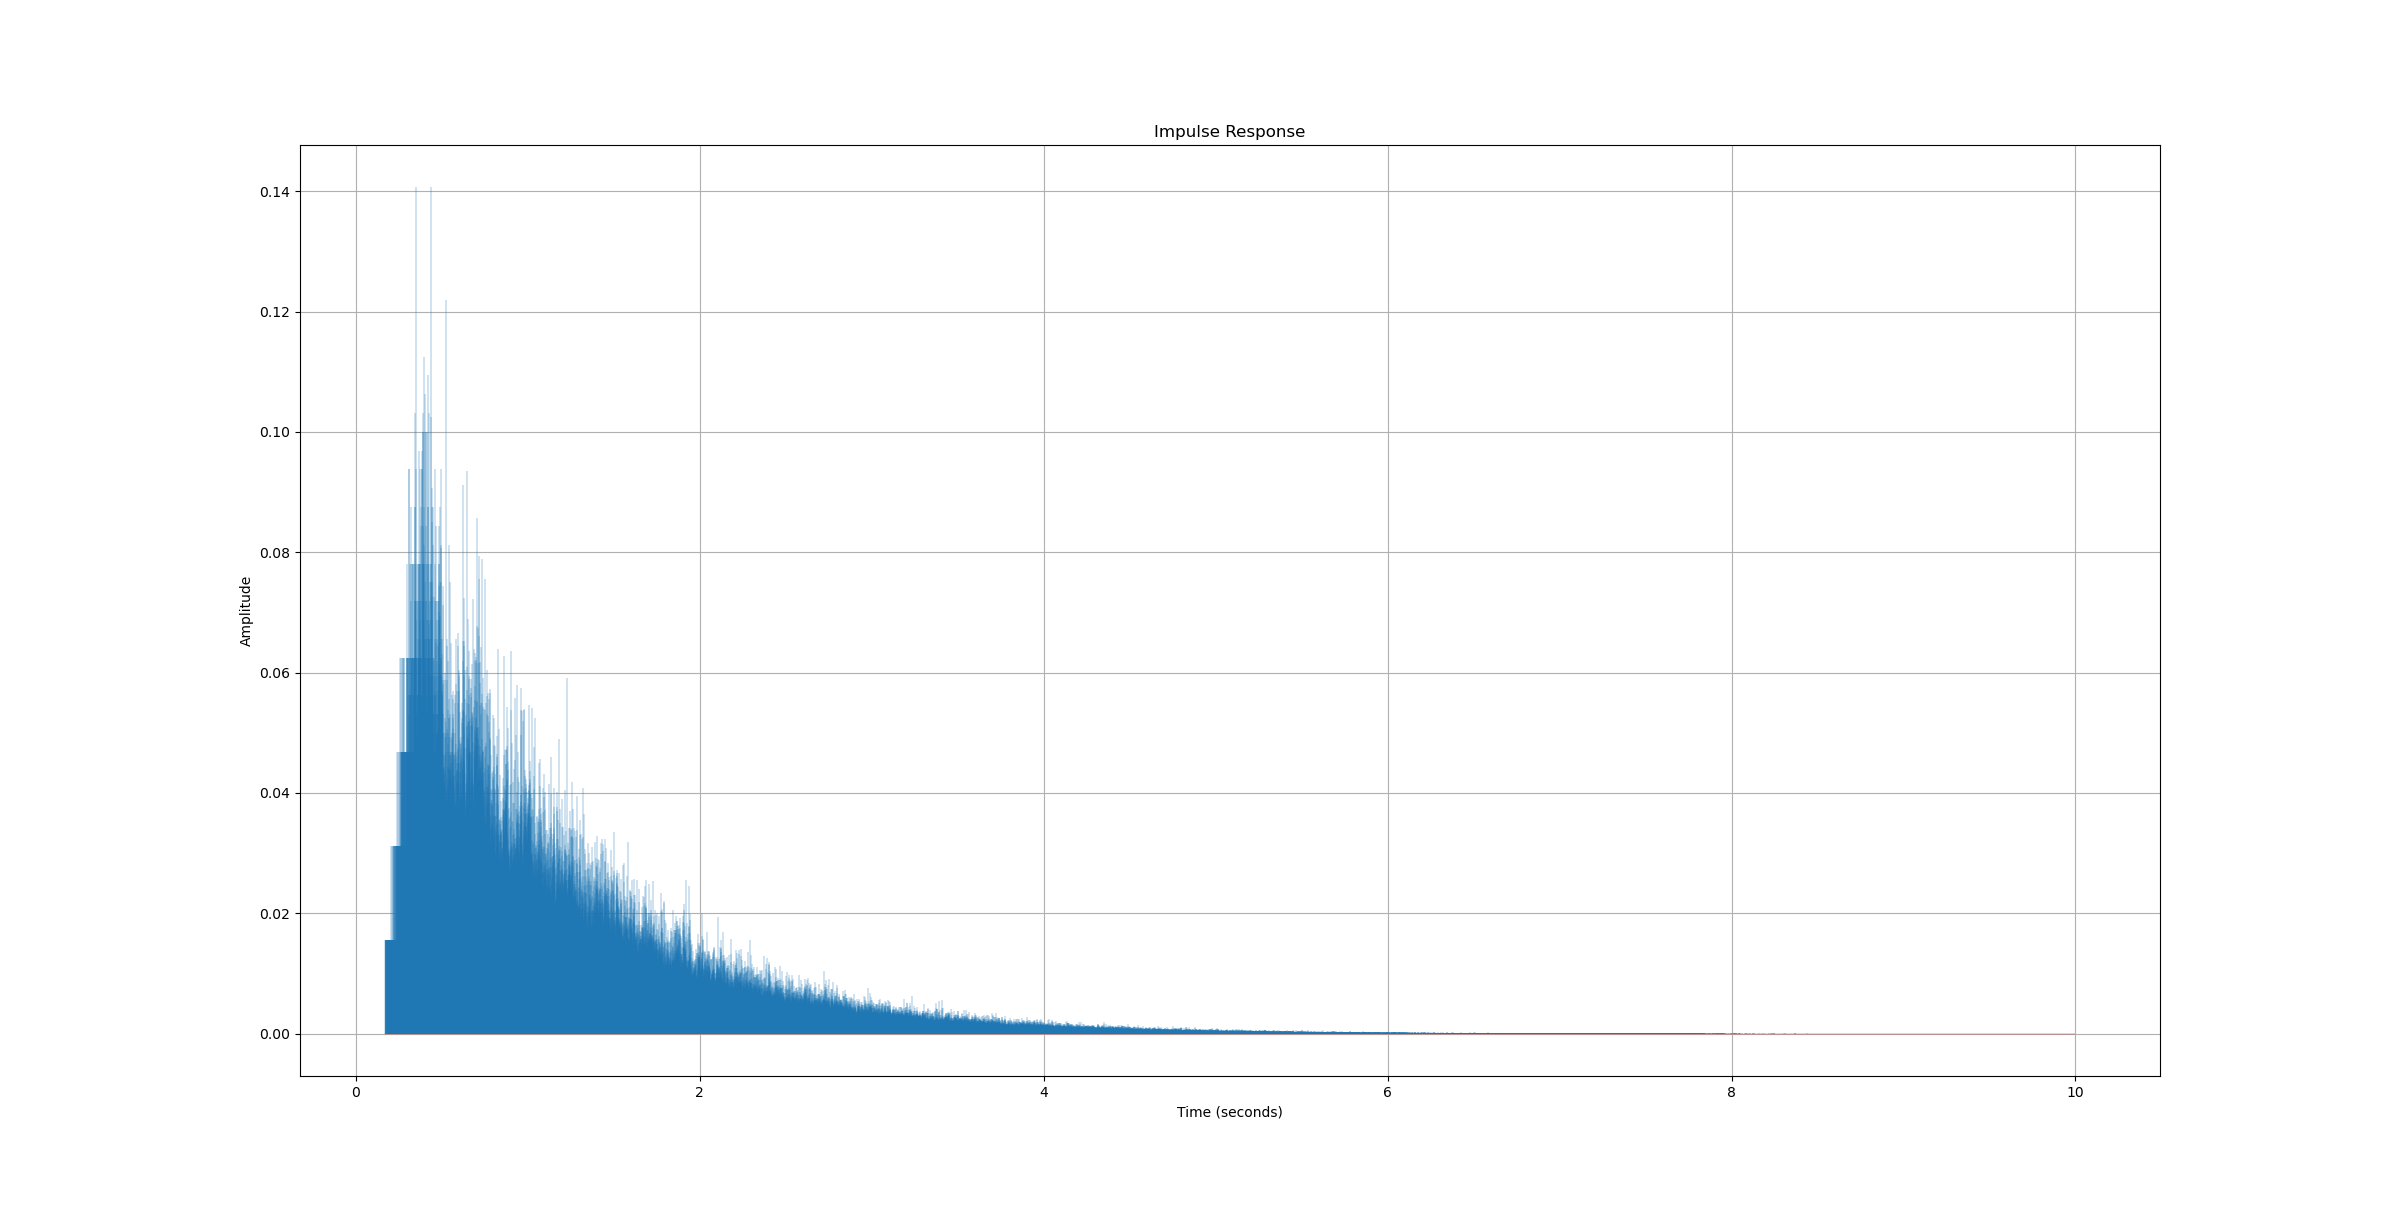
\includegraphics[width=\linewidth]{discussion/audio_effects/reverb/figures/reverb_stem_plot.png}
  \caption{Impulse Response of the Stem Plot}
  \label{fig:reverb-stemplot}
\end{figure}


Whereas, Figure \ref{fig:reverb-rmsenvelope} shows the RMS envelope curve in dB (\Cref{prompt:rms_plot_suggestion}) \cite{openai_chatgpt}. 
This also proves a natural energy decay. And in order for the audio to go silent, the time taken for the sound to decrease by 60 dB for 
a gain of 0.8 is estimated for 7 seconds. This also indicates the reverberation time (RT60) \cite{valimaki2012fifty} of around 7 seconds.

\begin{figure}[!htbp]
  \centering
  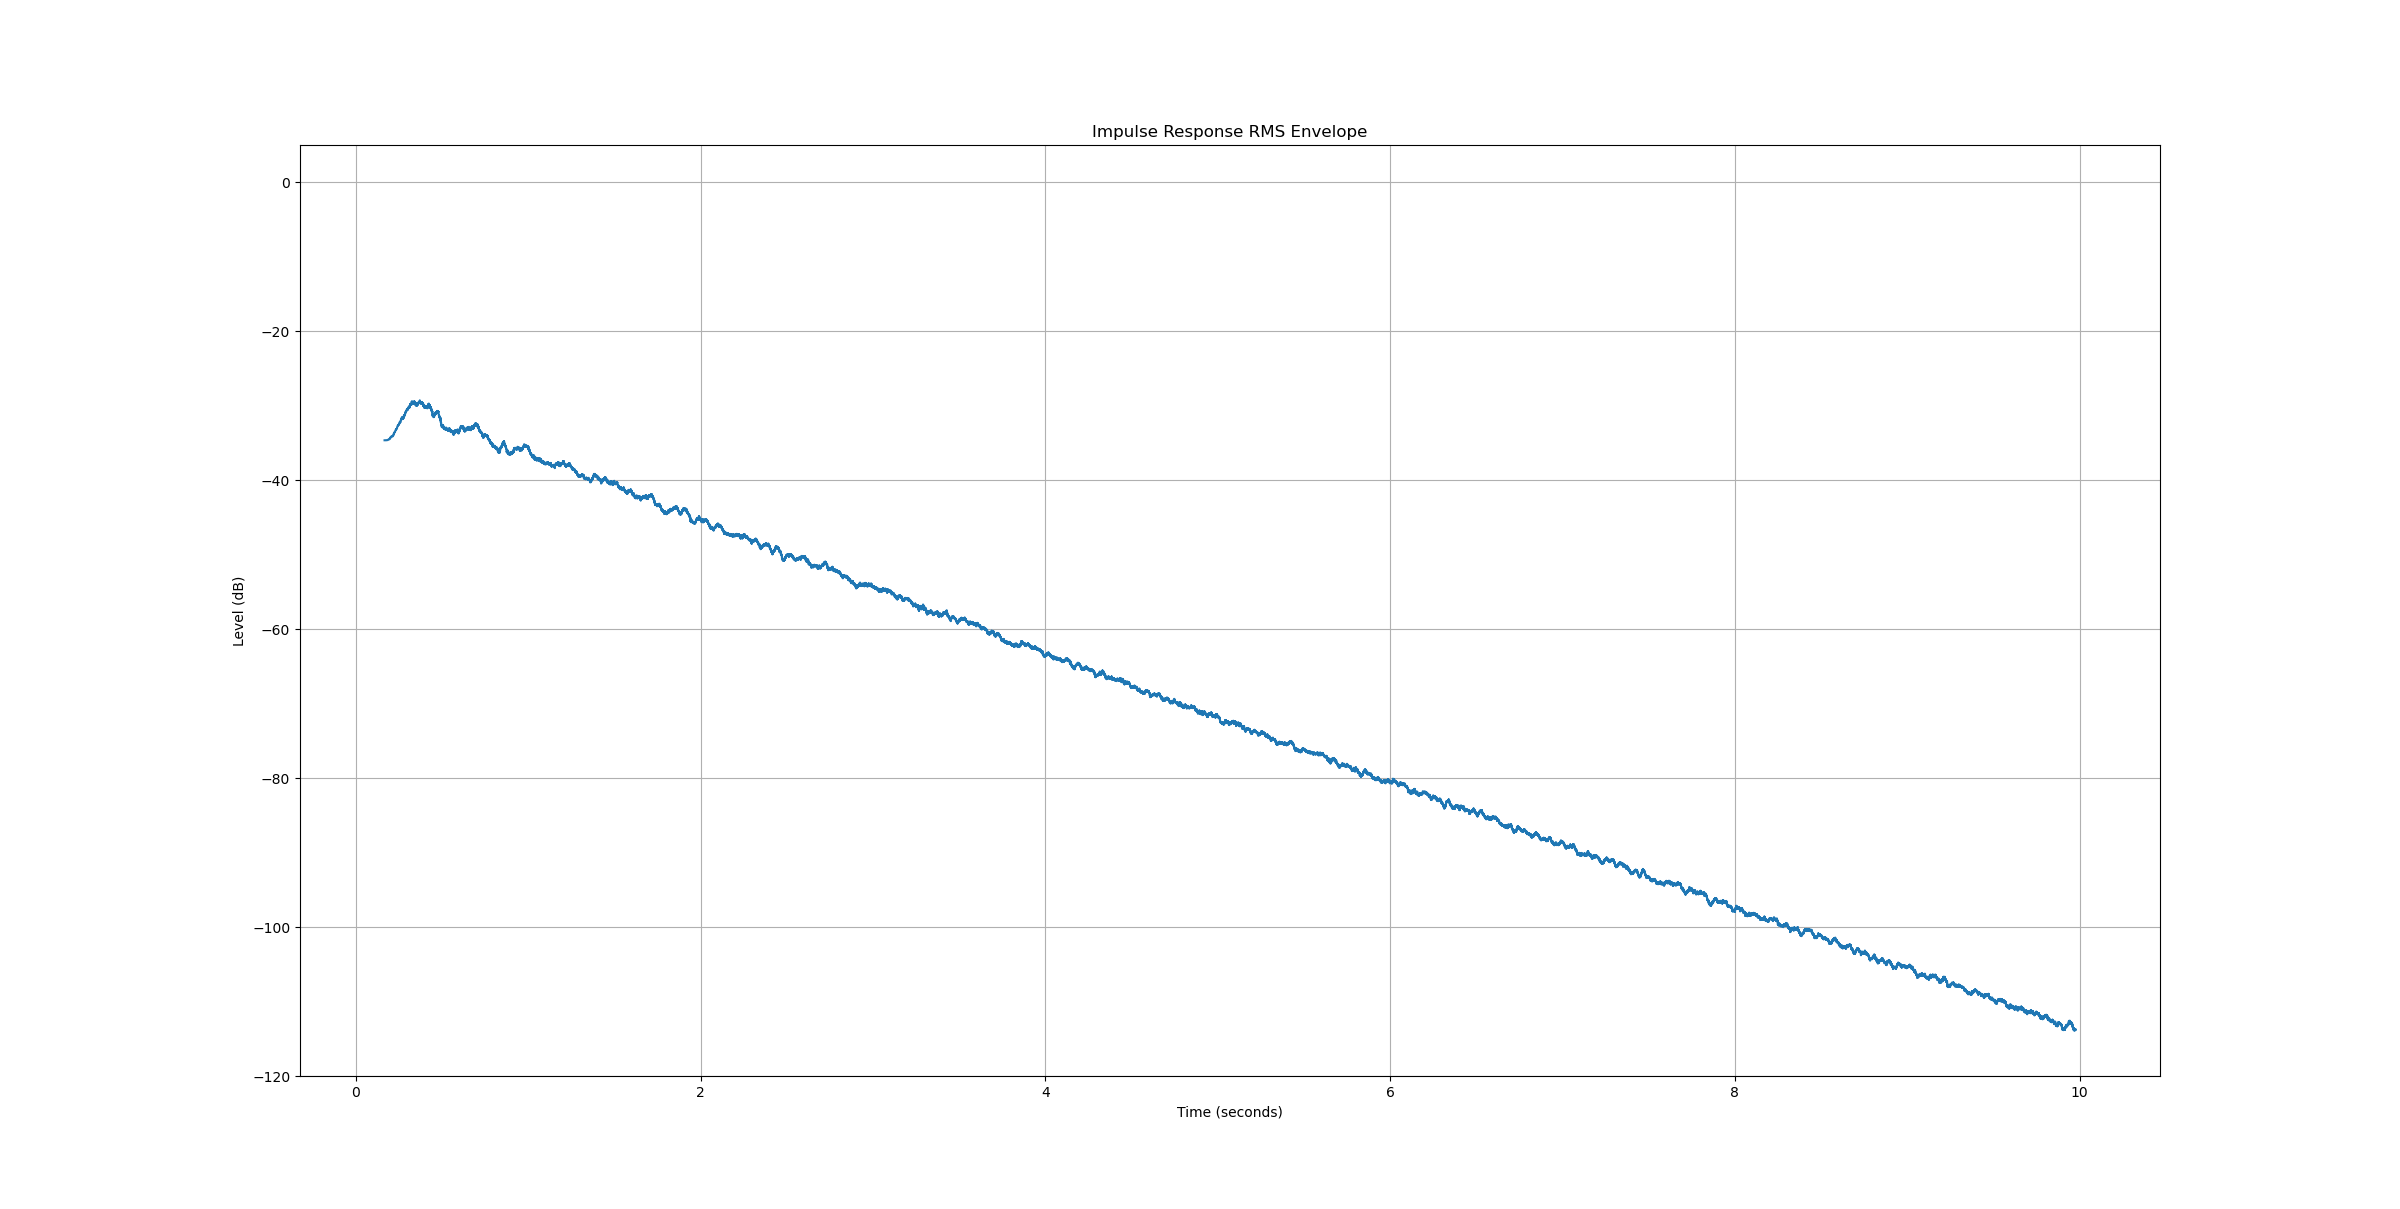
\includegraphics[width=\linewidth]{discussion/audio_effects/reverb/figures/amp_envelope_reverb.png}
  \caption{Impulse Response of the RMS Envelope Curve in dB \cite{openai_chatgpt}}
  \label{fig:reverb-rmsenvelope}
\end{figure}


This reverb is currently at bare minimum. Therefore, as discussed in Geriant's blog \cite{luff2021reverb},  
this can be further improved by adding a delay between the diffuser and the signal to put a time gap
between early reflection and late reverberations \cite{valimaki2012fifty}. Then, adding gentle LFO/modulation to delay
times gives the reverbed audio a ``supernaturally thick sound'', because some physical changes in the environment can
affect the timing in the reflections of sounds. And finally, shelving filter in the FDN can be added to absorb higher
frequencies, since they are absorbed much faster in real-life. All these improvements mentioned will make the reverbed
audio sound more realistic.

\paragraph{About Convolutional Reverb}
There is another way to make reverberation sound more accurate, which is the Convolutional Reverb, used in Logic Pro's
space Designer, for example \cite{apple2026spacedesigner}. It uses impulse responses recorded from real spaces. Then it 
takes that unique pattern of reflections to any audio source, therefore replicating spacious and diffused sound, when 
algorithmic reverb only depends on mathematical estimates. Even though it is more realistic, it is more CPU-heavy and 
less flexible any to parameter changes \cite{masteringbox2025convolution}. And most importantly, the captured impulse 
responses need to be recorded and cannot be done due to resource unavailability.

